\documentclass{article}
\addtolength{\oddsidemargin}{-1.cm}
\addtolength{\textwidth}{2cm}
\addtolength{\topmargin}{-2cm}
\addtolength{\textheight}{3.5cm}
\newcommand{\HRule}{\rule{\linewidth}{0.5mm}}
\makeindex

\usepackage{longtable}
\usepackage[pdftex]{graphicx}
\usepackage{makeidx}
\usepackage{hyperref}



\usepackage{changepage,lipsum,titlesec}% http://ctan.org/pkg/{changepage,lipsum,titlesec}
\titleformat{\section}[block]{\bfseries}{\thesection.}{1em}{}
\titleformat{\subsection}[block]{}{\thesubsection}{1em}{}
\titleformat{\subsubsection}[block]{}{\thesubsubsection}{1em}{}
\titlespacing*{\subsection} {2em}{3.25ex plus 1ex minus .2ex}{1.5ex plus .2ex}
\titlespacing*{\subsubsection} {3em}{3.25ex plus 1ex minus .2ex}{1.5ex plus .2ex}

\setlength\parindent{74pt}
 
\hypersetup{
	colorlinks=true,
	linkcolor=black,
	filecolor=magenta,      
	urlcolor=cyan,
}


% define the title
\author{Team now.next}
\title{ Software Requirements Specification}
\begin{document}
	\setlength{\parskip}{6pt}
	
	% generates the title
	\begin{titlepage}
		
		\begin{center}
			% Upper part of the page       
		
			\textsc{\LARGE Department of Computer Science}\\[1.5cm]
			\textsc{\Large COS 301 - Software Engineering}\\[0.5cm]
			% Title
			\HRule \\[0.4cm]
			%%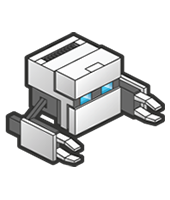
\includegraphics[width=0.05\textwidth]{./logo.png}\\[0.4cm] 
			{ \huge \bfseries Software Requirements Specification}\\[0.4cm]
			\HRule \\[0.4cm]
			% Author and supervisor
			\begin{minipage}{0.4\textwidth}
				\begin{flushleft} \large
					\emph{Authors:}
				\end{flushleft}
			\end{minipage}
			\begin{minipage}{0.4\textwidth}
				\begin{flushright} \large
					\emph{Student number:}
				\end{flushright}
			\end{minipage}
			
			\begin{minipage}{0.4\textwidth}
				\begin{flushleft} \large
					Vuyani {Shabangu}
				\end{flushleft}
			\end{minipage}
			\begin{minipage}{0.4\textwidth}
				\begin{flushright} \large
					\emph{}
					11171139
				\end{flushright}
			\end{minipage}
			
			\begin{minipage}{0.4\textwidth}
				\begin{flushleft} \large
					Sibusiso {Masemola}
				\end{flushleft}
			\end{minipage}
			\begin{minipage}{0.4\textwidth}
				\begin{flushright} \large
					\emph{}
					12270467
				\end{flushright}
			\end{minipage}
			
			\begin{minipage}{0.4\textwidth}
				\begin{flushleft} \large
					Sello {Thosago}
				\end{flushleft}
			\end{minipage}
			\begin{minipage}{0.4\textwidth}
				\begin{flushright} \large
					\emph{}
					13062060
				\end{flushright}
			\end{minipage}
			
			\begin{minipage}{0.4\textwidth}
				\begin{flushleft} \large
					Banele {Nxumalo}
				\end{flushleft}
			\end{minipage}
			\begin{minipage}{0.4\textwidth}
				\begin{flushright} \large
					\emph{}
					12201911
				\end{flushright}
			\end{minipage}
			
			\begin{minipage}{0.4\textwidth}
				\begin{flushleft} \large
					Aiden {Malan}
				\end{flushleft}
			\end{minipage}
			\begin{minipage}{0.4\textwidth}
				\begin{flushright} \large
					\emph{}
					12265731
				\end{flushright}
			\end{minipage}
			
			
			\vfill
			
		\end{center}
	\end{titlepage}
	\footnotesize
	%\input{declaration_of_originality.tex}
	\normalsize
	
	
	\pagenumbering{roman}
	\tableofcontents
	\newpage
	\pagenumbering{arabic}
	
	\newpage %Aiden malan
	\section{Introduction} 
	\begin{itemize} 
		\item The vision.
		\item The background.
	\end{itemize}
	
	\section{Vision}%%aiden
	
	
	\section{Background} %%aiden

	\newpage
	
	\section{Architecture Requirements}%Header
		\subsection{Architectural Scope}%%Aiden
		%Here just talk about overview of the architectural requirements. Just broadly what the quality of the product must be.
		
			\setlength{\leftskip}{45px}
				\lipsum[2]

		\subsection{Quality Requirements}%%Vuyani
			The following is a list of quality requirements that have been established by the product owner that the system must posses.
			\subsubsection{Stability}
				\setlength{\leftskip}{61px}
			 	In order to avoid costly damage to the drones, the system must be stable in that it must not be susceptible to failure. Should the system controlling the drone fail, the system should be able to guarantee the safe landing of a drone.
				
			\subsubsection{Performance}
			All non-reporting operations such as user registration, user login, mission submission, mission display, operator mission setup should not take longer than 0.5 seconds.
			
			The reporting operation where a report is given to the user after the drone has performed a mission should not take longer than 5 seconds after the report data has been made available to the system.
			
			Network overhead has not been included in these figures because that is beyond the control of the system.
			
			\subsubsection{Privacy}
			Drone missions should only be permitted in areas that are allowed by South African legislation pertaining to the flying of Unmanned Aerial Vehicles.
			
			The missions performed by the drones must also be permitted by South African legislation.
			
			\subsubsection{Security}
			It is important that this system adheres to the highest security standards because it will be storing personal user information such as physical addresses, as well as allowing for the control of drones which are expensive and can be dangerous if in the wrong hands. Therefore the system has ensure that:
			\begin{itemize}
				\item Personal user data such as password is encrypted to remain hidden from unauthorised users and operators.
				\item Only authentified users are able to access the system
				\item Users only perform what they are authorised to do (e.g. users can only see their own mission information, users cannot perform operator operations).
				\item Data sent between web portal client and server should be encrypted.
				\item Connectivity to drones should only be limited to authorised and authentified users and system components
			\end{itemize}
			
			\subsubsection{Scalability}
			The system should scale up in order to be able to support a growing number of users, drone missions (which may be simultaneous), and drones. It should also scale as the data (user data, drone data and reporting data) held by the system increases.
			
			\subsubsection{Integration}
			The system must be able to interface with different drones.
		\subsection{Integration and Access Channel Requirements}%%Sello
		%Here just speak about what the system is expected to integrate with. Write about how it is suppose to be accessable to 			%web for users and operators.  It must also be able to interact with different types of drones.
		\subsubsection{Integration}
		The system has to work with the ArduPilot system. This ArduPilot system has to be conected to the PixHawk flight controller hardware. The drone operating system should be able to deploy missions to as many different drones as possible.
		\subsubsection{Access Channels}
		The system is supposed to have a portal for drone users and operators which should be accessible through the internet. In the later stages of development, after completion of the web version of the system, the system could also possibly be made into an Android application.
		\subsection{Architectural Constraints }%%Banele
		%Talk about the constraints that we might have in producing the architecture that they have asked for.
	\section{Architectural patterns}%%Sibusiso MVC, layered
	%Write that we are using a hybrid of MVC and Layered pattern (MVC to support the web part of the system, and layered to 		%support the intergability required by the part of the system that talks to the drones)
	\section{Architectural Tactics}%%Banele
	%use the same tactics that we spoke about in the presentation, discuss them more in detail
	\section{Access and Integration channels}%%Sello
	%This time, you are writing about the how we will meet the intergration requirements that you wrote about earlier. Write about how 	%we will use a HTTPS REST API to interact with the web portal. Talk about our layered approach to interacting with the drones; 	%our system->drone interfacing object -> adrupilot -> pixhawk -> drone.
	\subsection{Integration Channels}
	The drone user or operator portal will generate a text file. From this text file, an external drone operator will read the contents of the text file and enter the mission details into the ArduPilot software. The PixHawk flight controller hardware needs to be physically connected to the computer running the ArduPilot software via USB. The PixHawk flight controller keeps a stack of all ordered missions. The flight controller will then send the mission instructions to the drone via a wireless connection.
	\subsection{Access Channels}
	A HTTPS RESTful API will be used to handle the communication between the web client (the drone user or operator portal) and the web server. 
	\section{Technologies}%%Sibusiso
	%List and describe all the technologies we will be using, including why we are using them. Make sure for each one you mention 	%how it solves an architectural requirement.
	%MEAN Stack (Mongo, ExpressJS, AngualrJS, NodeJS), Mongoose (for ORM), Heroku Server, Travis for CI... and others
	
	
	
	
	
	
\end{document}
